\documentclass[12pt]{article}
\usepackage{graphicx}
\usepackage{caption}
\usepackage{amsmath}
\usepackage{bibtopic}
\usepackage{hyperref}
\usepackage{calrsfs}
\usepackage{float}

\setlength{\parskip}{1em}

\begin{document}

\setlength\parindent{0pt}
\title{Raw Audio Music Generation Using Deep Neural Networks}
\author{Fabian Stahl}


\maketitle

\tableofcontents

\newpage
\section*{Abbreviations}
\begin{center}
\begin{tabular}{l l}
\textbf{CNN} & Convolutional Neural Network \\
\textbf{DCGAN} & Deep Convolutional Generative Adverserial Networks\\
\textbf{GAN} & Generative Adversarial Network \\
\textbf{GRU} & Gated Recurrent Unit \\
\textbf{KLD}  & Kullback–Leibler Divergence\\
\textbf{LSTM} & Long Short-Term Memory \\
\textbf{MIDI} & Musical Instrument Digital Interface \\
\textbf{MLP} & Multilayer Perceptrons \\
\textbf{NLL} & Negative Log-Likelihood \\
\textbf{ReLU} & Rectified Linear Unit \\
\textbf{RNN} & Recurrent Neural Network \\
\textbf{VAE} & Variational Autoencoder \\
\textbf{VRNN} & Variational Recurrent Neural Network \\
\end{tabular}
\end{center}
\newpage


\section{Motivation}
Music can be found in almost every movie, video game or public location.
Its targeted use can change people's mood, encourage buying decisions or add context to accompanying content.
However, composing, recording and mixing music is a creative process that takes a lot of time and skill to master.
This poses the question if pleasing music can be generated autonomously.

Deep neural networks have been known to solve a wide range problems.
This paper will introduce three different network architectures to generate sample based music, show how they can be trained and compare the results.


\section{Related Work}
% midi
In the field of audio generation there is a wide variety of approaches.
Most of them work with symbolic music representations, such as ASCII-text, musical scores or spectrogram data.
Especially the MIDI format is commonly used, a binary format specifying musical notes.
This makes the format very slim and easy to work with.
MIDI-based approaches include e.g. Generate Adversarial Neural Networks with convolutions layers ~\cite{yang2017midinet, mogren2016c, mogren2016c}, Variational Autoencoders paired with Long Short-term memory cells~\cite{roberts2018hierarchical, tikhonov2017music, hennig2017classifying} and Recurrent neural networks with restricted Boltzmann machines \cite{boulanger2012modeling}.
However, musical nuances like tonal colors, scratch and breath noises or intonations are necessary to make most music genres more realistic.
While sometimes these small subtle variations are not even perceived consciously, their absence can affect the overall impression. 
Having MIDI output only, the musical interpretation, (the raw audio sent to the sound port), is up to an external MIDI synthesizer that cannot produce these nuances.

There are commercial music streaming services that claim to provide generated music that fits the customer's mood.
The most prominent of them being brain.fm~\cite{brain.fm} and \cite{mubert}.
However, the brain.fm algorithm only learns certain tasks, such as arranging motifs over long timescales, while melodies, instrument choices and chord progressions are pre-composed by humans.
Mubert also uses handcrafted single instrument MIDI loops, but generates some MIDI layers using decision trees, random forests and musical analysis.
The services music is limited to electronic genres only, which narrows musical variety.
While the application developers like to emphasize the machine learning aspect, their algorithms are not fully autonomous.
The two biggest reasons for that could be the high complexity of generating music sample by sample, especially with real time constraints, as well as the ineptitude of the synthesized music for commercial use.




\section{SampleRNN}
Recurrent Neural Networks (RNNs) are used to process sequences of data.
Output data is not only based upon input data, but also on a hidden state vector, that encodes previous input.
RNNs consist of arrays of small memory units.
While the original \emph{vanilla cells} were prone to the vanishing gradient problem, more advanced structures like Long Short-Term Memory cells (LSTMs) and Gated Recurrent Units (GRUs) are able to learn to keep important information and forget redundant or irrelevant previous input.

In audio data correlation can exist between neighbouring samples as well as between samples that are more than thousand frames apart.
Mehri et al. states that common RNNs don't scale very good with a very high temporal resolution and proposes to use multiple hierarchical stacked RNNs with different temporal resolutions to capture all audio features~\cite{mehri2016samplernn}.
This model is called \emph{SampleRNN}.
Originally tested only for piano music, \cite{zukowski2018generating} and \cite{carr2018generating} showed, that SampleRNN is especially good to generate loud music genres, like Metal and Dark Ambient.
This makes the SampleRNN a promising candidate for music generation.

The implementation used in this work was built on top of a project called \emph{Deepsound-project}~\cite{samplernn-git}.
However, in a few cases this version differs from the original proposal.
The main differences to the original implementation include
\begin{itemize}
 \item works with an arbitrary number of frame-level tiers
 \item upsampling layers prior to RNN cells
 \item 1D convolutions with stride 1 instead of fully-connected layers (equivalent operations, but better performance)
\end{itemize}



\subsection{Architecture}
The (Deepsound-project) SampleRNN consists of multiple hierarchically stacked \emph{frame-level modules} and a single \emph{sample-level module}.
Each frame-level module is an RNN that generates a conditioning vector for the next lower tier based on a state vector that summarizes previous input.
The same audio data is passed to all Modules, but while the number of chunks increases with the lower tiers, the chunks itself become smaller, i. e. the clock rate gets faster.

At the bottom of the model is a single \emph{sample-level module}.
It puts the combined conditioning vector from above into consideration as well as the raw audio samples to generate a probability distribution for each chunk.




\subsection{Training}
To allow an efficient training of the model, truncated backpropagation through time (TBTT) is used.
Since it is computational very expensive to propagate gradients back after a full song, training on shorter sub-sequences of 8 seconds is much more feasible.
The initial state vectors of all GRUs was learned.

\begin{figure}
    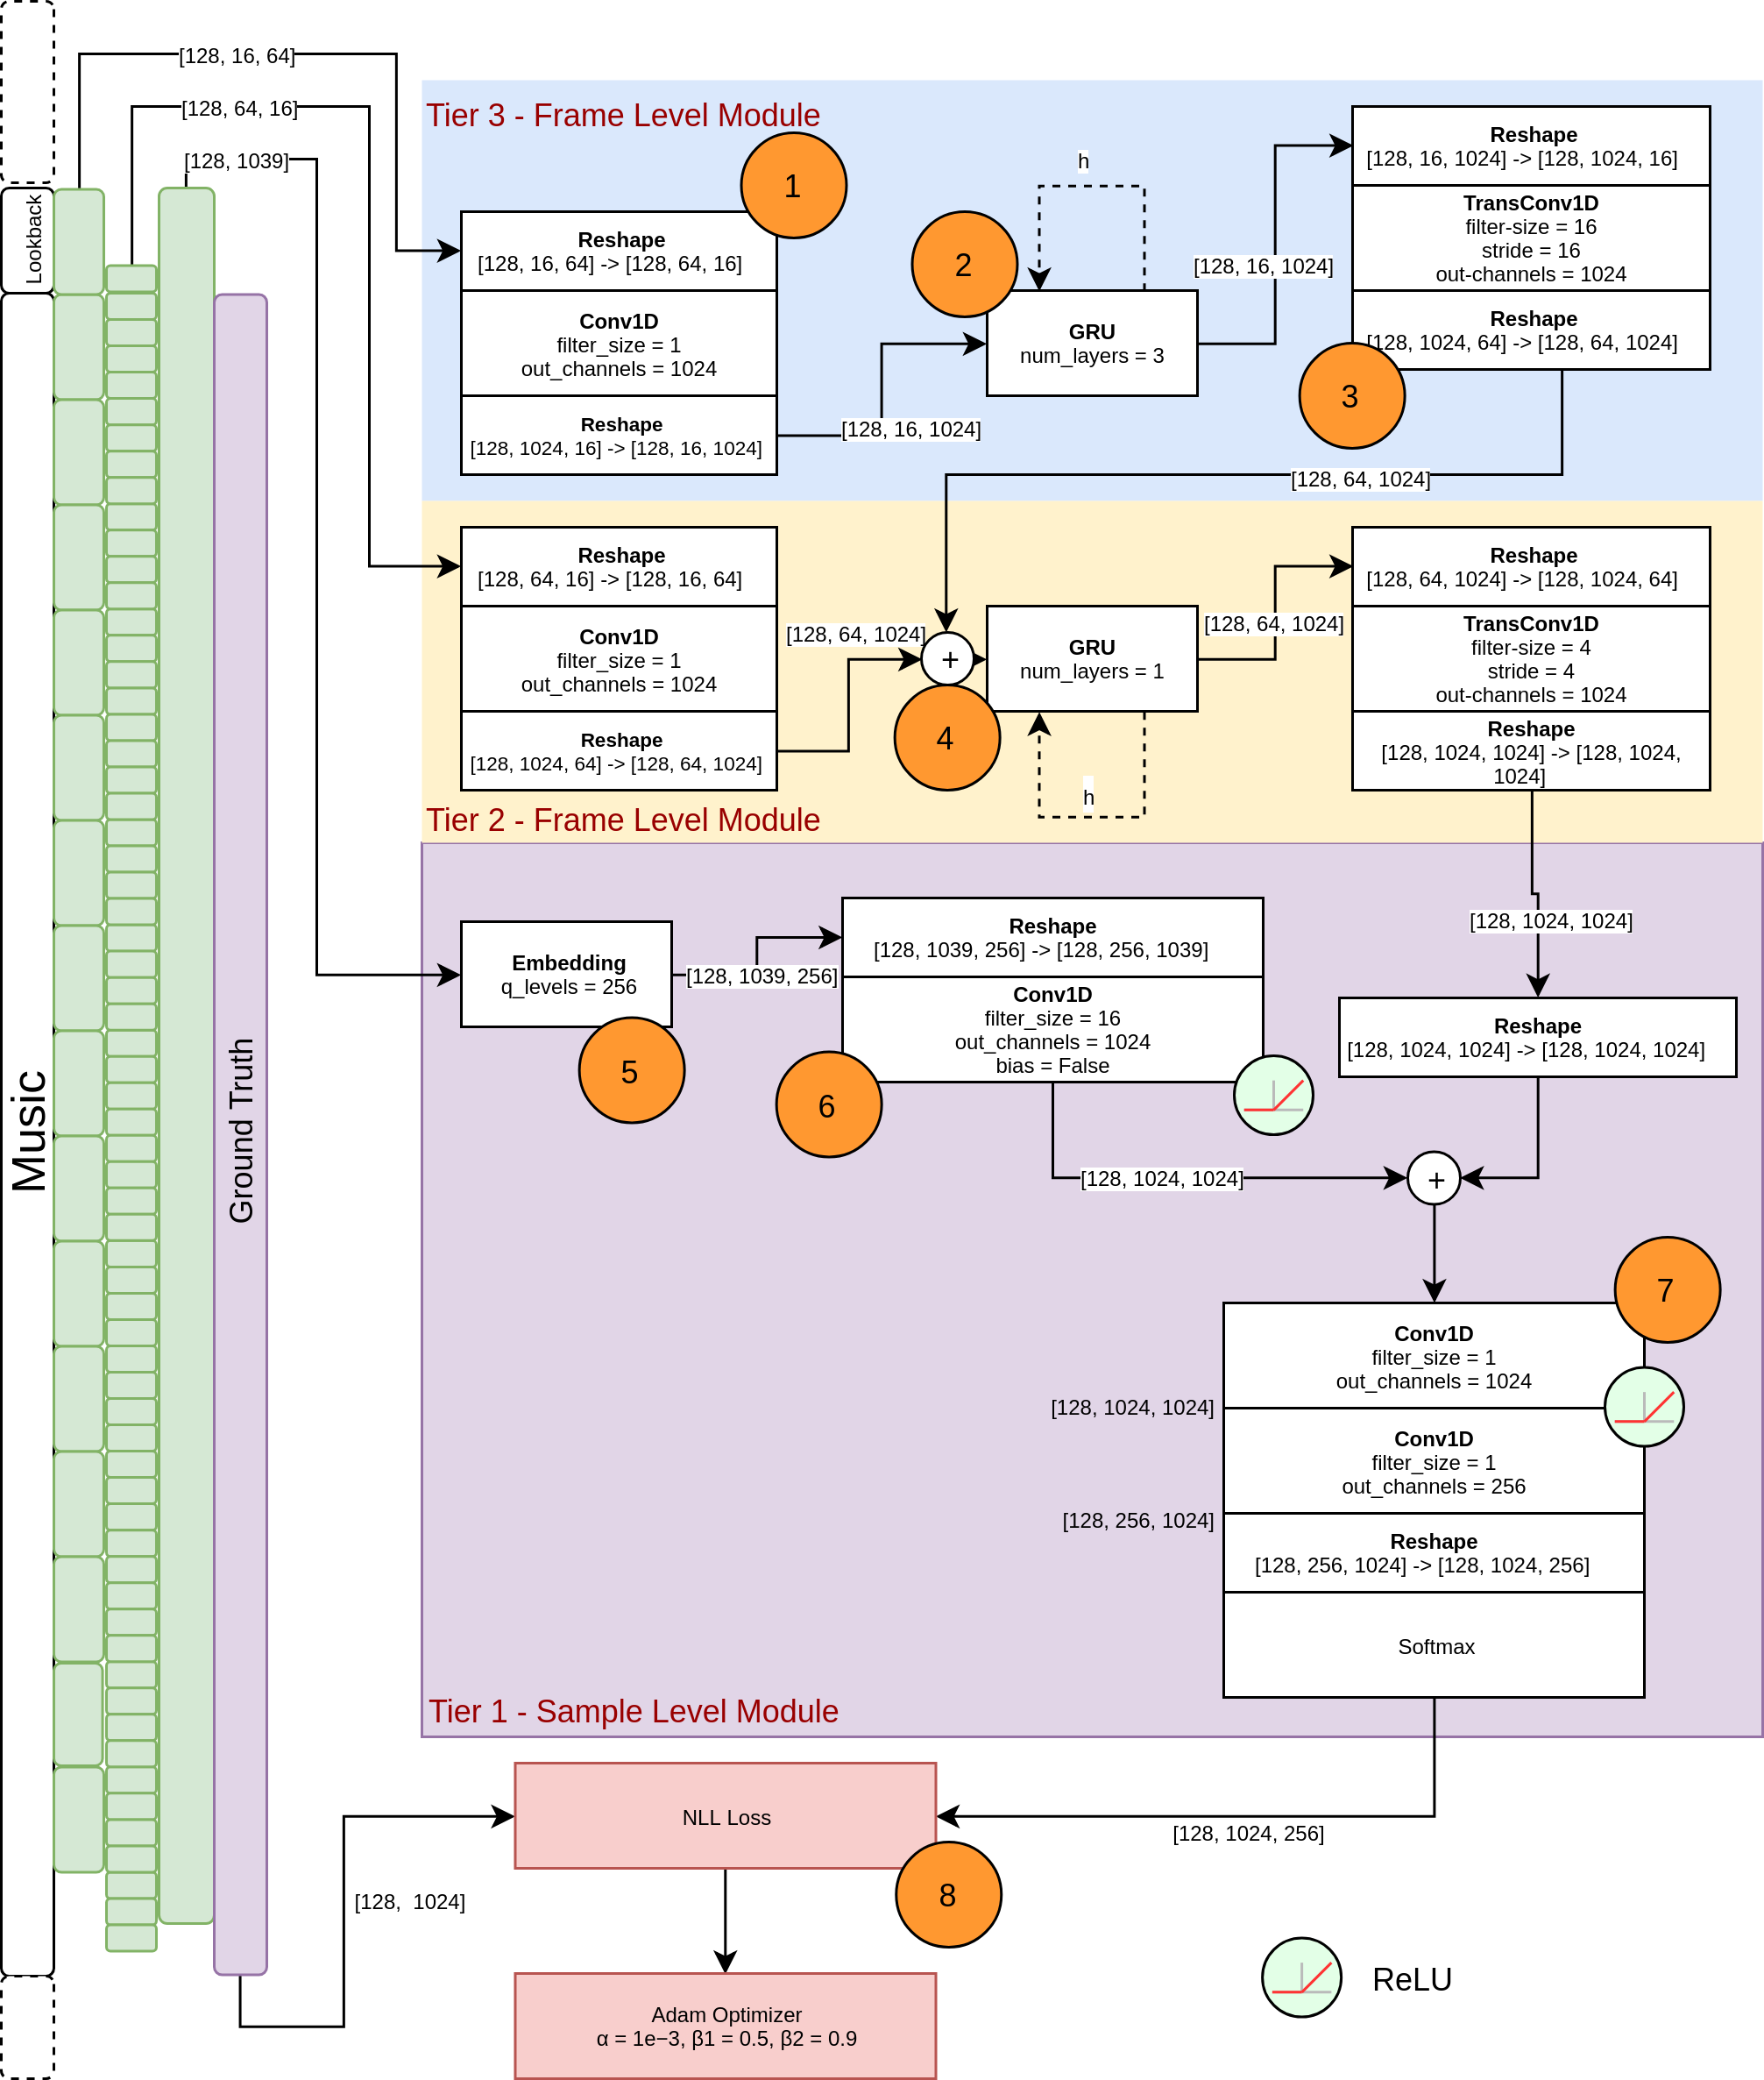
\includegraphics[width=\textwidth]{img/samplernn-arch.png}
    \caption{The SampleRNN architecture with the best output results consists of two stacked frame-level modules and a sample-level module. All tiers receive the same input but depending on the tier it is chunked differently. The output is a q-way Softmax which means for each of the 128 batch items and for each of the 1024 chunks a probabilities for 256 output values are assigned.}
    \label{fig:samplernn-arch}
\end{figure}

Figure \ref{fig:samplernn-arch} shows a training cycle of a SampleRNN trained with the following parameters:
\begin{center}
\begin{tabular}{ r | l | l }
variable name & value & description \\
\hline
frame sizes & 16, 4 & numbers of frame-level chunks per upper tier chunk\\
sequence length & 1024 & how many samples to include in each training step\\
quantization levels & 256 & number of bins in quantization of audio samples\\
num rnns & 3 & number of stacked GRUs per frame-level \\
dim & 1024 & dimension of the state vectors $h$, neurons in sample-level \\
learning rate & 0.001 & \\
batch size & 128 & \\
sample rate & 16000 & \\
\end{tabular}
\end{center}

First the upper frame-level module chunks the input data into 16 chunks, each containing 64 samples. 
Using a 1D convolution with stride 1 each 64 dimensional sample chunk is expanded to a 1024 dimensional sample chunk (1).
These chunks are fed into three stacked GRUs, that predict the follow up sequences based upon a state vector $h^1_t$ (2).
To be able to pass the condition vectors to the next lower tier with a faster clock rate, a transposed 1D convolution helps to upsample 16 to 64 chunks (3).
The middle tier repeats step 1, but uses a smaller clock rate (64 chunks, each with 16 samples) and adds the expanded result to the conditioning vector from above (4).
The signal than passes the middle tier GRU and upsampling layers.
The sample-level module first quantizes the whole input sequence to 256 bins and maps them to a real-values vector embedding (5).
This signal is passed through a 1D convolution to match the conditioning signal from the middle tier (6).
The combined signal passes a Multilayer Perceptron (expressed with 1D convolutions) as well as a Softmax layer to calculte 256 probability vaues for each batch item for each chunk (7).
According to \cite{mehri2016samplernn} a discrete output distribution using a q-way Softmax yields better results than a continual distribution using for example Gaussian Mixture Models.
Finally the output signal is compared to the ground truth data and the negative log likelihood (NLL) is calculated.
Based on this score the Adam optimizer adjusts the models parameters (8). 


SampleRNN experiments were stopped after no more validation progress was achieved.
On a NVIDIA RTX2080 GPU, this took about 35 hours and almost the full 8Gb RAM.




\subsection{Generation}
At generation time the sample-level module is run repeatedly, where each sample is fed back into the model.
Conditioning vectors from the frame-evel modules are refreshed using a lower clock rate if enough samples are generated to feed a new non-overlapping input chunk to the RNNs.





\section{VRNN}
\subsection{Idea}
Another approach to generate sound data is the \emph{Variational Recurrent Neural Network (VRNN)}, proposed 2016 by Chung et al.~\cite{chung2015recurrent}.
The architecture was trained on the tasks of sound generation as well as handwriting.
However, experiments for the first only included training with speech datasets and non-linguistic human-made sounds like coughing and screaming.
This poses the question if the VRNN can be used to generate music as well.

Chung et al. states that there is an issue in the way that RNNs model output variety, since it is often the only source of true randomness to draw values from an output probability density.
Data that is both highly variable and highly structered can be hard to model this way.
On the one hand small input variations should lead to potentially very large variations in the hidden state vector $h_t$, on the other hand, different high level structures need to be mapped to distinct state vectors as well.
This forces the network to compromise between the encoding of low-level and high-level features.
The main idea of the VRNN is to extend a recurrent neural network with latent random variables, therefore improving the representational power of the model.
Such high-level variables are commonly used in VAEs to model multimodal conditional distributions, approximating real world data variety~\cite{kingma2013auto}.
Chung et al. proposes to extend the VEA model by inducing temporal dependencies using the hidden state vector of a RNN across neighboring timesteps.



\subsection{Training}

% Normalisierung eingangsdaten: To-do


\begin{figure}
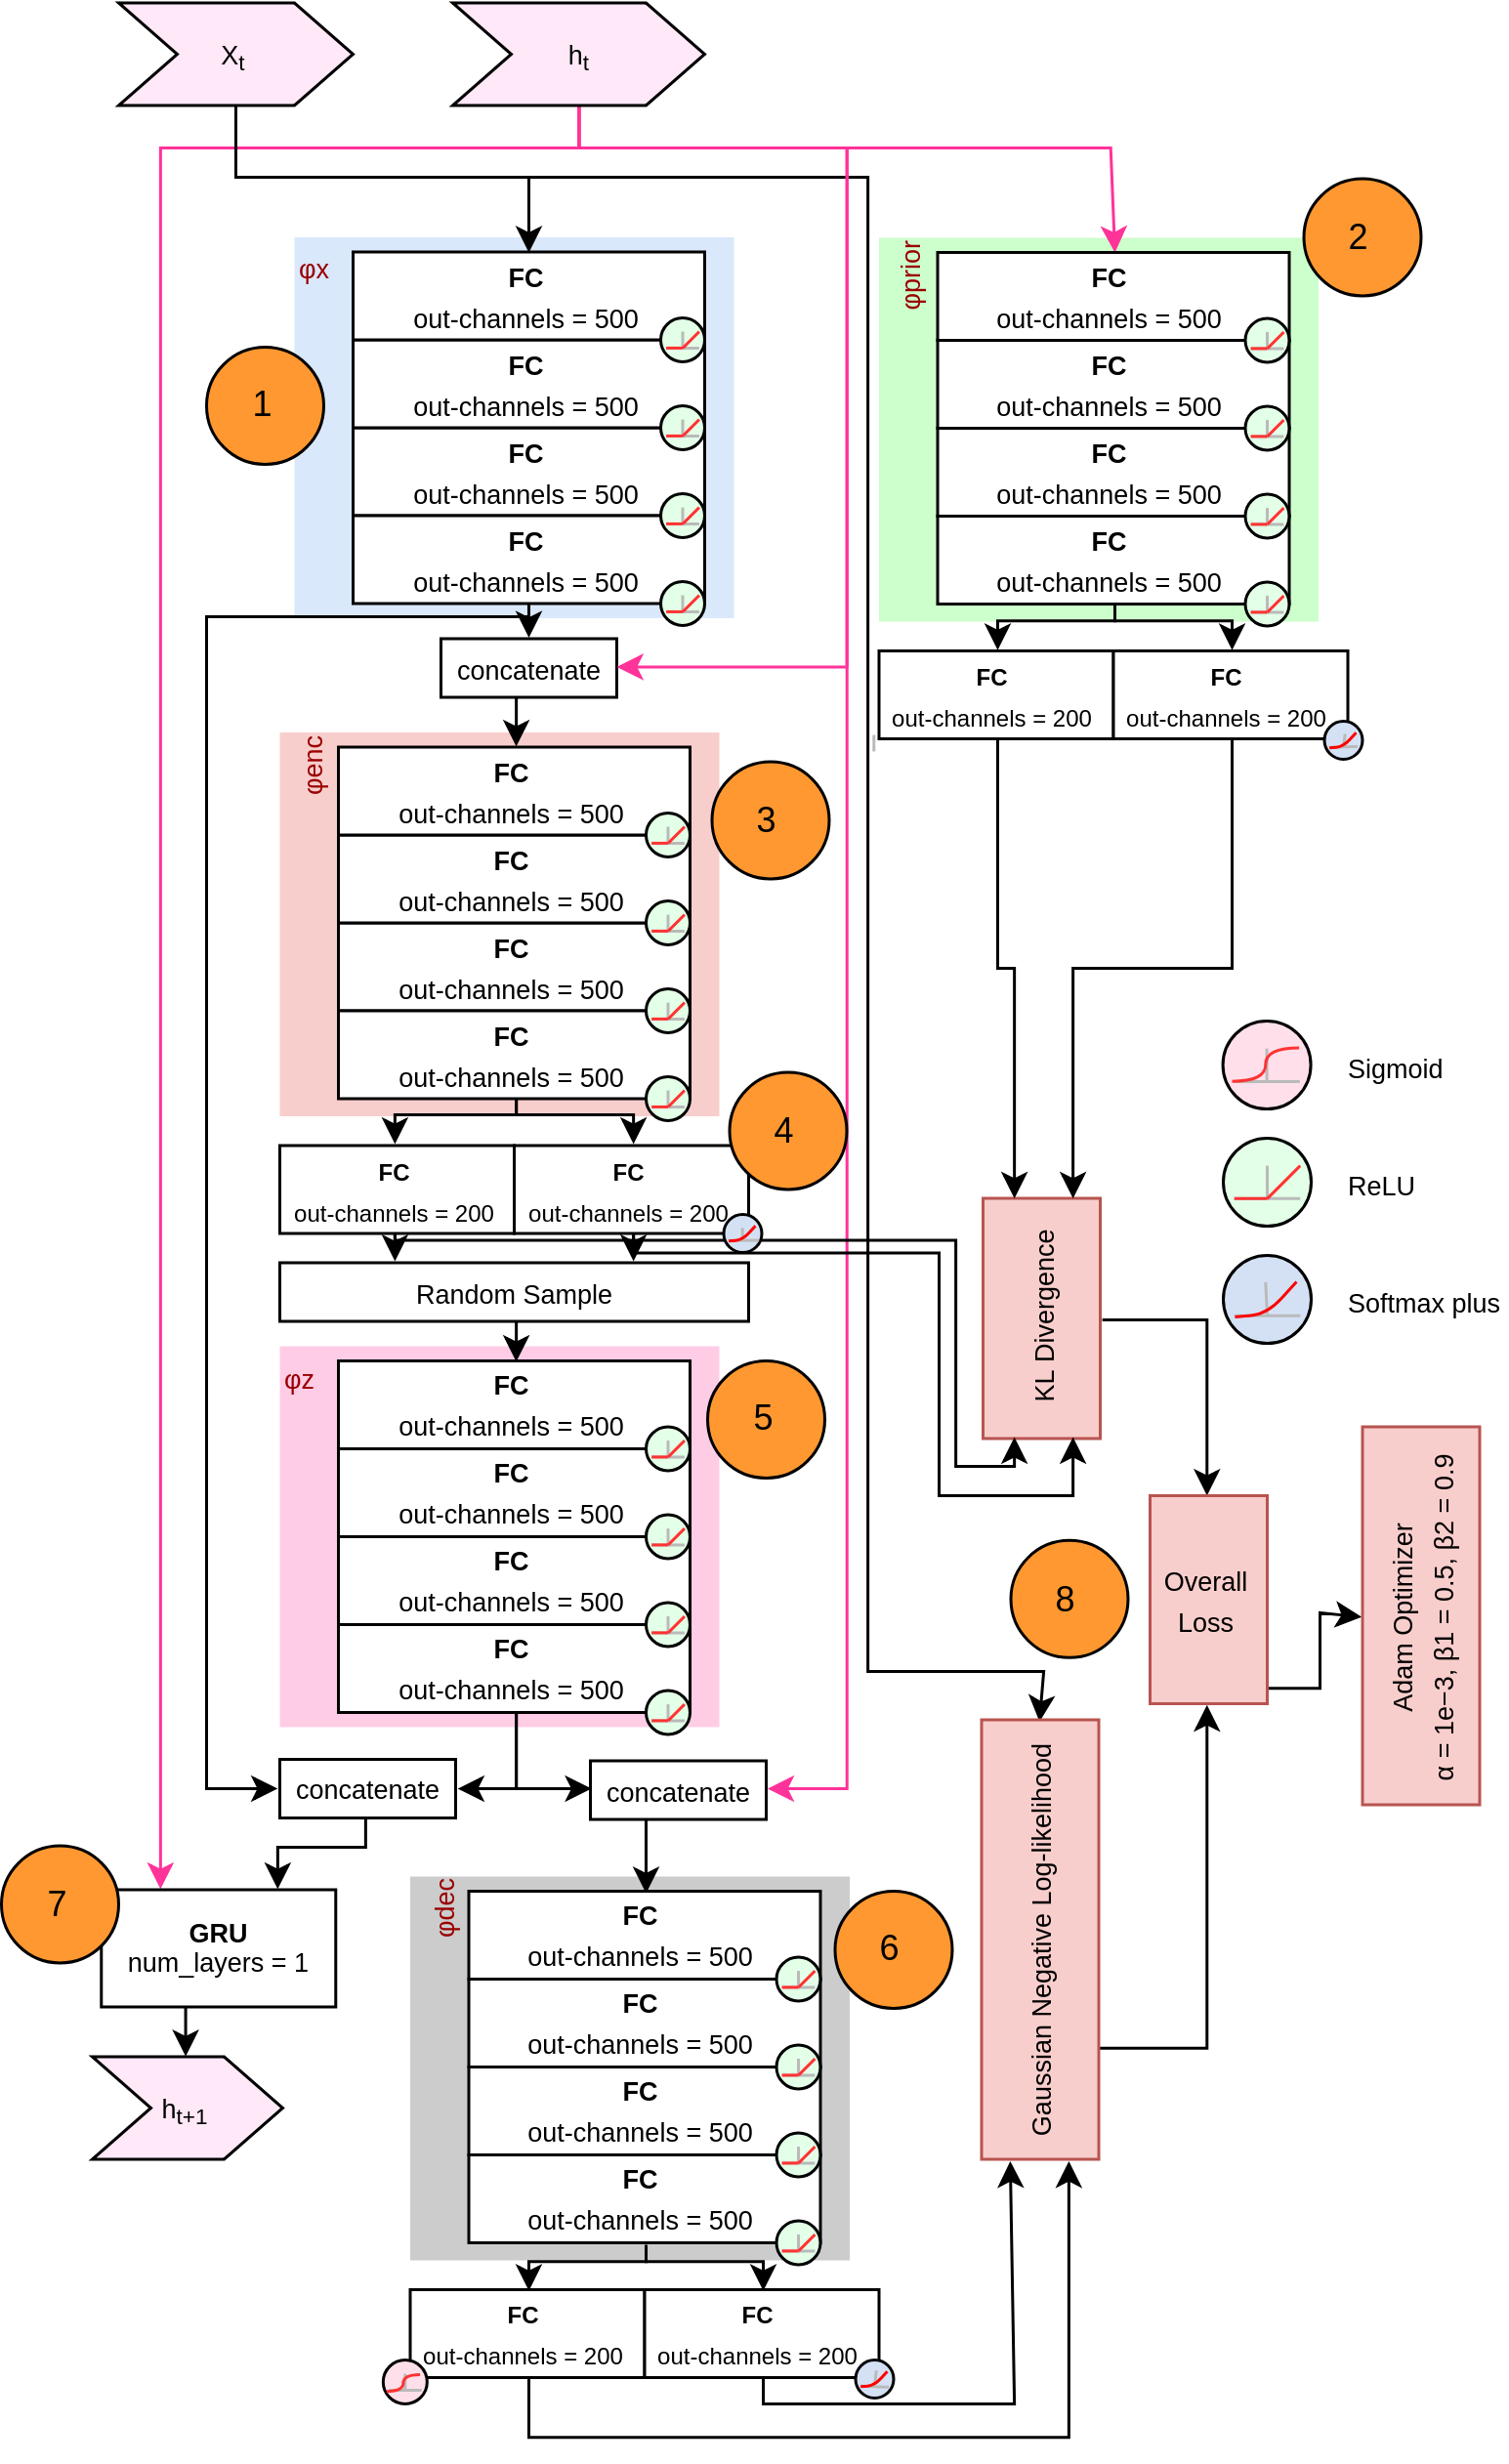
\includegraphics[width=0.9\textwidth]{img/vrnn-arch.png}
\label{fig:vrnn-arch}
\caption{VRNN architecture} % To-DO!
\end{figure}



Figure \ref{fig:vrnn-arch} shows all necessary steps for a training cycle.
First the raw audio data is passed through $\varphi^x$ to extract features from $x_t$ (1).
According to \cite{chung2015recurrent} $\varphi^z$ as well as $\varphi^x$ are crucial to learn complex sequences.
Since the Kullback–Leibler divergence (KLD) is used to make the outputs of $\varphi^{prior}$ and $\varphi^{enc}$ as similar as possible, the prior needs to be included in the model.
It handles the state vector $h_t$ and generates both $\mu^{prior}$ and $\sigma^{prior}$(2).
The encoder $\varphi^{enc}$ is used during training only.
It takes $\varphi^x$ and the state vector $h_t$ and calculates $\mu^{enc}$ and $\sigma^{enc}$ (3).
Now $z$ is drawn from $\mathcal{N}(\mu^{enc}, \sigma^{enc})$ (4).
Another network $\varphi^z$ is used to find features in $z$ (5).
The decoder is used to replicate the input data $x$.
It therefore takes the concatenated $\varphi^z$ and $h_t$ into consideration (6).
Also, $z$ and $h$ are passed to the RNN to determine a new state vector $h_{t+1}$ (7).
Lastly the overall loss is calculated (8).
It is composed of the KLD from $\varphi^{prior}$ and $\varphi^{dec}$ to make them similar, as well as a reconstruction loss that compares $\mu^{dec}$ to $x$. 



% Describe p, q, ...

%conditional prior / generative model - p(x | z)
%approximate posterior / inference model - q(z | x)
%prior over latent random variables - p(z)


The model can be trained by minimizing the Kullback–Leibler divergence (KLD) - first term - and maximizing the likelihood of an $x$ given a $z$ - second term).
This can be seen as adding a regulizer to a simple auto encoder to ensure that the generated distributions have a certain form.
$$
E_{\mathbf{z} \le T | \mathbf{x} \le T} = \left[ \sum_{t=1}^T -(KL(q(\mathbf{z}_t | \mathbf{x}_{\le t}, \mathbf{z}_{<t}) || p(\mathbf{z}_t | \mathbf{x}_{<t}, \mathbf{z}_{<t})) + log(p(\mathbf{x}_t | \mathbf{z}_{\le t, \mathbf{x}_{<t}}))) \right]
$$

The KLD between the two distributions $Q$ and $P$ with respect to $Q$ is a measurment of similarity between two distributions.
Since the probabilistic Encoder $q(z|x)$ is used to approximate the hard to compute posterior $p(x|z)$, $Q$ needs to be as similar to $P$ as possible.
This means that the KL divergence needs to be minimized, which is identical to maximizing the lower variational bound~\cite{kingma2013auto}. 


In this work Gaussian distribution models are used to model real world variability.
However, In theory the model can be trained using any probability distribution, like the Gaussian Mixture Model (GMM).

For all experiments the follwing parameters prooved to be most effective
\begin{center}
\begin{tabular}{ r | l | l }
variable name & value & description \\
\hline
frame length & 200 & numbers of samples per input chunk\\
num rnns & 1 & number of stacked GRUs per Frame-Level \\
clip & 0.1 & clips gradient to this length to avoid gradient explosion \\
dim $\phi^x$, $\phi^{dec}$ & 600 & number of hidden units \\
dim $\phi^z$, $\phi^{enc}$, $\phi^{prior}$ & 500 & number of hidden units \\
dim $h$ & 2000 & number of hidden units in the state vector $h$ \\
learning rate & 0.0003 & \\
batch size & 128 & \\
sample rate & 16000 & \\
\end{tabular}
\end{center}

All input sample have been normalized using the global dataset mean and standard deviation.


% Implementierungsdetaills
Since the original source code was using the Theano ML library, I cloned a public PyTorch implementation~\cite{VRNNgit}.
However, I found out, that I needed to make quite many adaptions to fit the original version.
The biggest changes include a new data loader class, adding the correct error function, using more dense layers in all components and make the code more GPU-friendly. 



\subsection{Generation}
Conditioned on the input vector $h_t$, $\varphi^{prior}$ is used to calculate $\mu^{prior}$ and $\sigma^{prior}$ values so that the latent variable $z$ can be drawn from $\mathcal{N}(\mu^{prior}, \sigma^{prior})$.
To extract features from $z$ the signal passes $\varphi_z$.
Finally $\varphi^{dec}$ is used to decode $z$.
Since the decoder is trained with Gaussian KLD loss, the decoder yields $\mu^{dec}$ and $\sigma^{dec}$.
Output values can be drawn from $\mathcal{N}(\mu^{dec}, \sigma^{dec})$.
However, in the original implementantation $\mu^{dec}$ is used as output.

To produce sound of more than 200 samples, $h_t$ needs to be adjusted and fed back into the model.
In order to do that $x$ is drawn from $\mathcal{N}(\mu^{dec}, \sigma^{dec})$ and passed through the feature xtractor $\varphi^x$.
Finally the encoded $x$ and $z$ are passed to the RNN and $h_{t+1}$ can be calculated.












\section{WaveGAN}
In 2014 Goodfellow et al. introduced a new approach to train networks called Generative Adversarial Networks (GANs)~\cite{goodfellow2014generative}.
Such networks consist of a generator and a discriminator sub-network.
While the discriminator tries to distinguish between real and generated data, it is the generators task to fool the discriminator into thinking its output is real.
Both networks are trained simultaneously and try to outperform each other.

While GANs have been used widely for tasks related to images, there are only few approaches using audio data.
Donahue et al. presented two GAN approaches to generate sound data called \emph{WaveGAN} and \emph{SpecGAN}~\cite{donahue2018adversarial}.
Both models are adaptions of a model class called Deep Convolutional Generative Adverserial Networks or DCGANs, first proposed by Radford et al.~\cite{radford2015unsupervised}.
The SpecGAN works with spectrogram images that are processed by the network in a similar way to normal images.
However, the final conversion from image to sound data is known to be problematic, since a lot of noise is induced.
The second architecture, the WaveGAN, is a flattened adaption of the original DCGAN model using 1D convolutions on raw audio samples.
Both models have the same number of parameters and numerical operations.
However, neither strategy has been tested with music data.
Since SpecGANs lossy conversion poses difficulties beyond the actual AI model, only the second approach will be presented here.

Unfortunately the original model description is only capable to generate about a second of audio.
By adding one more transposed convolution layer to both the encoder and the decoder, and increasing the number of intermediate output channels, the models generating capacity can be increased to about 4 seconds, possibly enabling whole musical motifs. 
This expanded model can be found on the authors GIT repository~\cite{donahue2019wavegan}.



\subsection{Architecture}
See figure \ref{fig:WaveGan-arch} for a visualization of the graph with parameters.
The generator network is trained to map a low-dimensional latent vector $z$ to a high-dimensional data output.
First the network applies a fully connected layer with $512d$ output nodes to $z$, where $d$ is used to adjust the models size.
The output vector is then reshaped, since an additional dimension is needed for the sound channel.
The signal then passes 5 transposed 1D convolution layers with stride 4 and ReLU activation functions in between as well as a Tanh function at the end.

The decoder is basically a mirrored generator with a few exceptions.
Instead of ReLUs, Leaky ReLUs with $\alpha=0.2$ are used in between convolution layers.
Also a new kind of layer, called Phase-Shuffle, is introduced here. 
Since the generators transposed convolution is known to produce artifacts, the discriminator may learn to find generated samples based on these artifacts instead of conducting a broad content analysis.
Shifting the vector randomly up to $n$ times in a circle can prevent this learning behavior.





\subsection{Training}

\begin{figure}
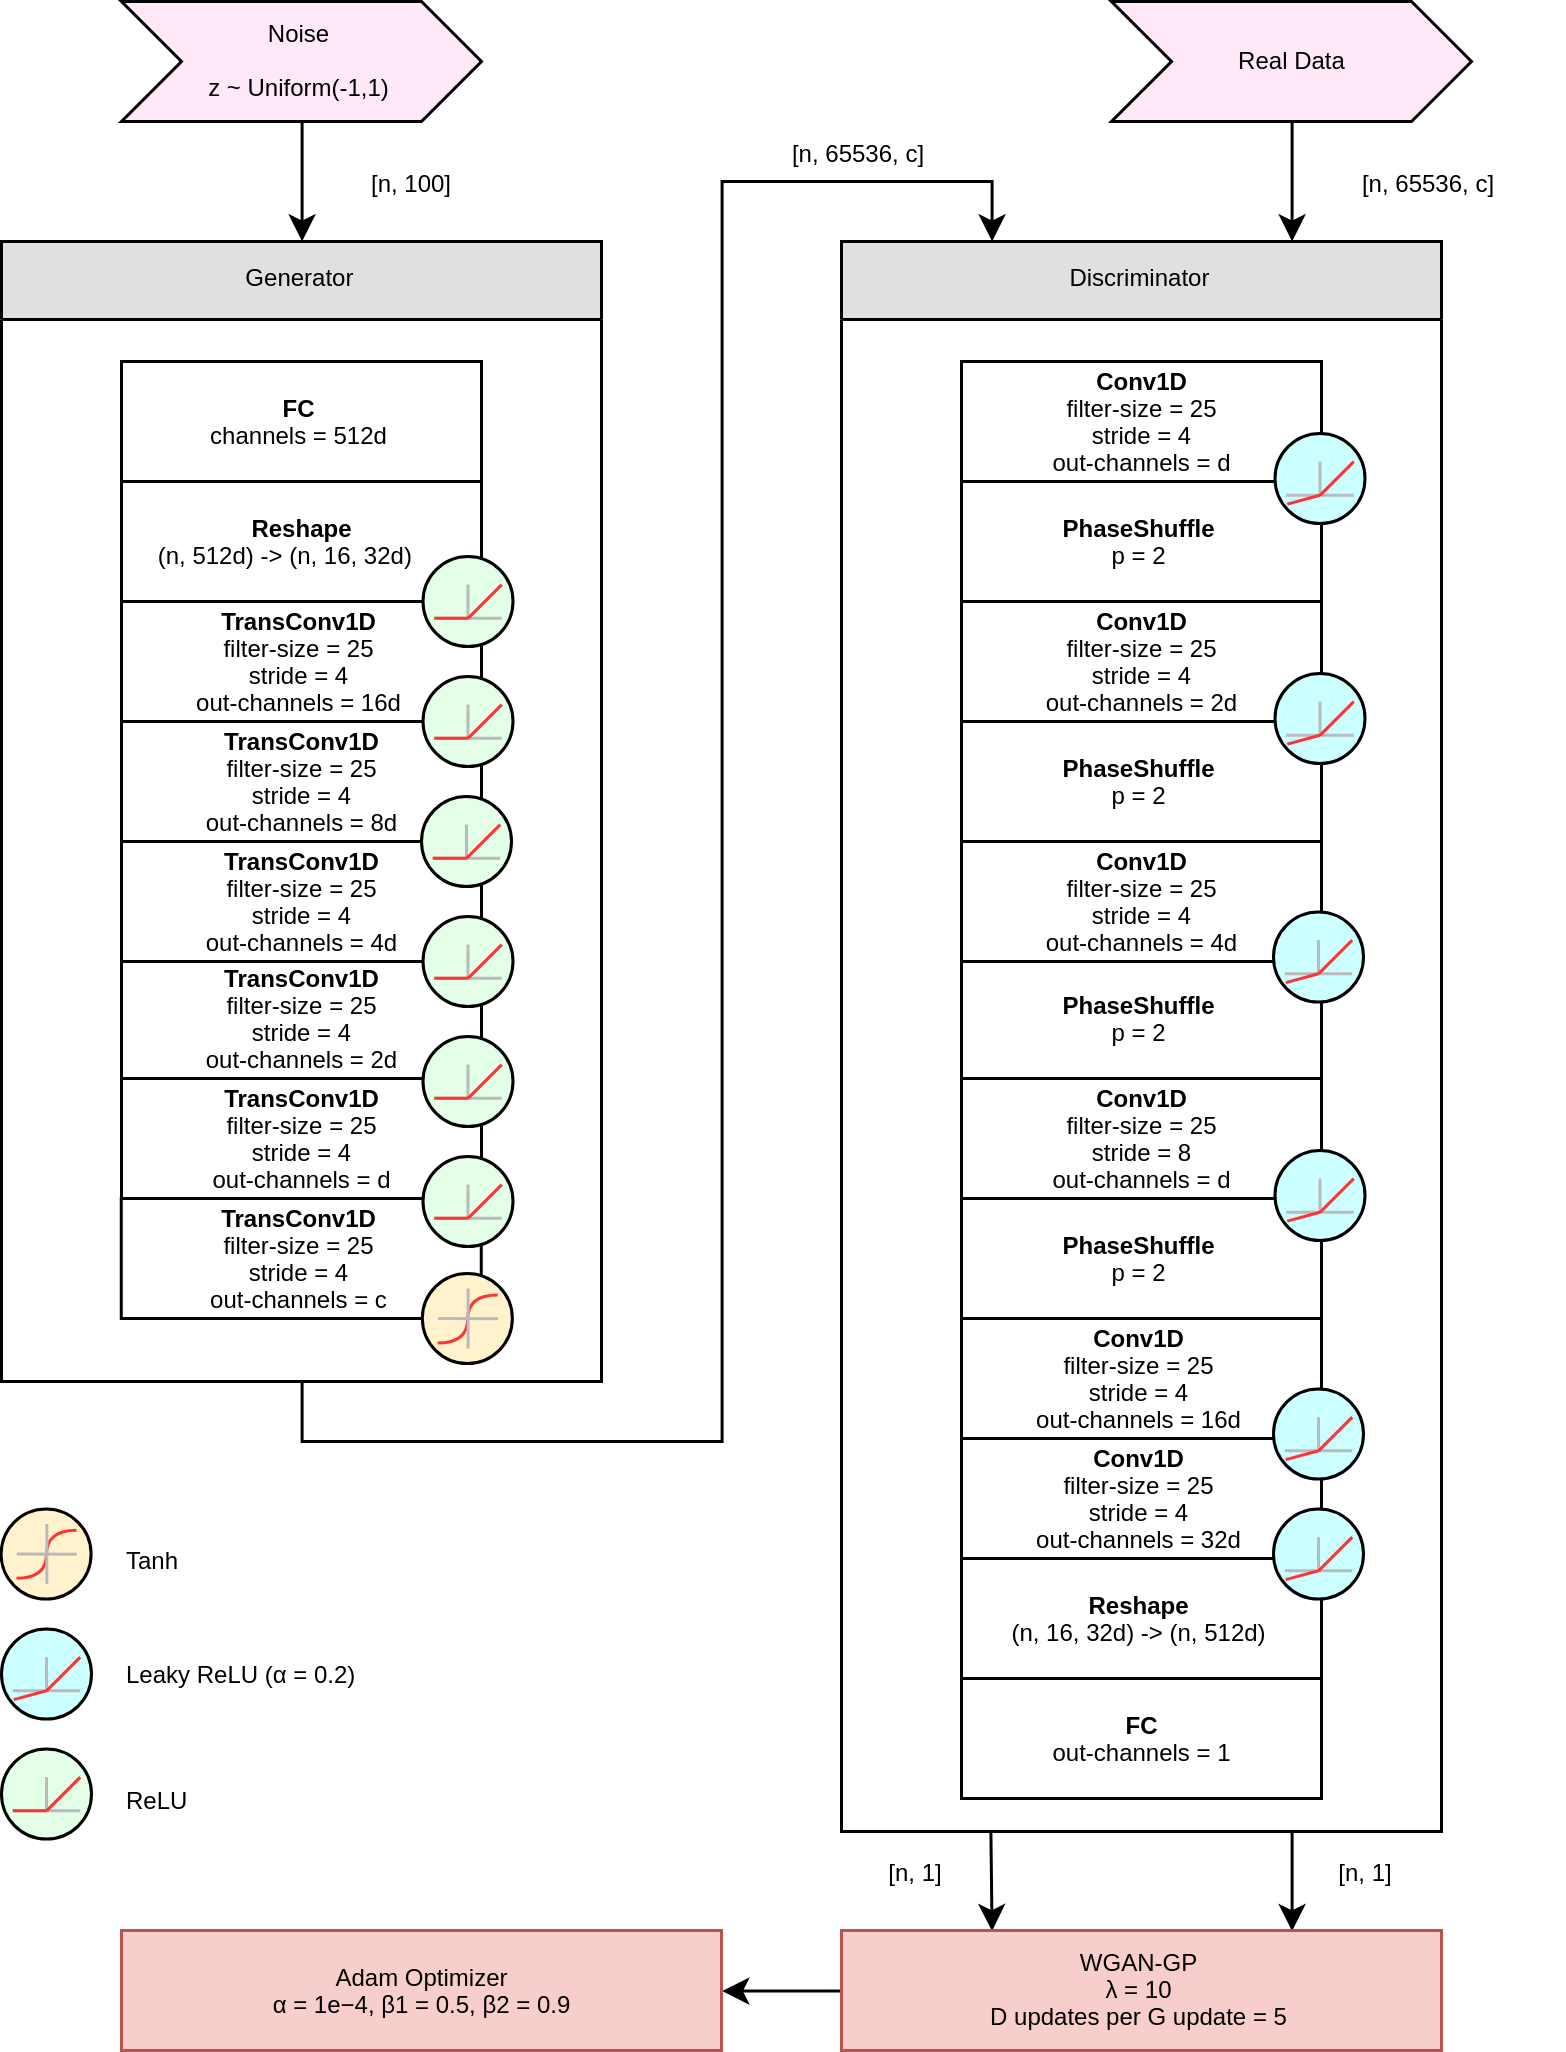
\includegraphics[width=0.9\textwidth]{img/wavegan-arch.png}
\caption{While the generator tries to produce realistic data using transposed convolution layers based upon a latent noise vector $z$, the discriminator tries to distinguish between generated and real data. The parameter $d$ can be used to adjust the models size. $n$ is the batch size and $c$ is the number of output channels.}
\label{fig:WaveGan-arch}
\end{figure}

Training GANs can be seen as a two player minimax game. 
While the generator $G$ is trained to minimize the following value function, the discriminator $D_w$ is trained to maximize it.

$$
V_{WGAN}(D_w, G) = E_{x \sim P_x}[D_w(x)] - E_{z \sim P_z}[D_w(G(z))]
$$

The network is trained using the Wasserstein-GAN Gradient Penalty, or short \emph{WGAN-GP}, strategy.
That means, that instead of predicting probabilities, the discriminator is trained to assist computing the wasserstein or earth movers distance between the distribution of generated data and distribution of real examples.
However, minimizing this measure is only possible if the discriminator function is 1-Lipschitz, which can be done by enforcing a gradient penalty.
For more details on the WGAN-GP strategy see~\cite{gulrajani2017improved}.

In most WaveGAN experiments training was stopped in between $40.000$ and $50.000$ steps since no more progress was achieved.
On a NVIDIA RTX2080 GPU, this took about a day and 7 of 8Gb RAM.
All other parameter choices are similar to \cite{donahue2018adversarial}.
Adam Optimizer with $learning rate = 1e-4$, $\beta^1 = 0.5$ and $\beta^2 = 0.9$ was used for both discriminator and generator.
The model was trained using both a batch size $b$ and a scale factor $d$ of $64$.








\section{Experiments}
SampleRNN, VRNN and WaveGAN have been rained on
\begin{itemize}
 \item piano music (Felix Mendelssohn: Lieder ohne Worte, about 2 hours)
 \item instrumental metal (Intervals: The Way Forward + A Voice Within (Instrumental Version) + In Time, 1 hour and 53 minutes) 
 \item hip-hop (Cypress Hill: Cypress Hill, 46 minutes)
\end{itemize}

For SampleRNN the music was split into 8 second, for VRNN into 0.5 second and for WaveGAN into 4 second chunks.
It should be mentioned that the music format used in all experiments is mp3.
Among other tricks to reduce its file size, this format relies on psychoacoustic phenomenas.
For example, frequencies that cannot be heard by the human ear or are overshadowed by previous louder sound are cut out.
However, these features might be important for AI models to learn music generation.
Future work might investigate how training with raw uncompressed music data influences the models accuracy.


Please listen to the provided audio examples of all experiments.
They can be found on the repository page \textbf{sound-results.html}.





\textbf{SampleRNN}\\
Despite its relative complicated architecture, the SampleRNN learned to produce first musical features like drum hits, scratches and screams after only about 5 minutes of training.
It takes much more training to reduce noise and generate more complex features like guitar riffs.
In my experiments SampleRNN was able to produce the most clean sound compared to the other models.
However, sample quality varies strongly even after days of training.
With the Hip-Hop dataset the model even completely regressed to produce random sounds.
These quality variations were also described by \cite{carr2018generating} who advised to restart training if output samples during training remain bad.
Future work should investigate how to avoid this unpredictable behavior.

Another drawback of the SampleRNN is the long music generation time since every generation cycle outputs a single sample that needs to be fed back into the model.
With the architecture described above it takes about half an hour to generate 5 minutes of audio.
However, assuming that there is enough memory, increasing generation batch size does not affect the overall generation time since it can be parallelized.



\textbf{VRNN}\\
The VRNN model proved to be the worse candidate in terms of output quality and training difficulty.
Compared to the SampleRNN, that generates assignable instrument sounds after a few epochs, the VRNN training progress is very slow, yielding sawtooh-like waves most of the time.
Also exploding gradients and huge loss values cause the training to crash despite of gradient clipping with a threshold of $0.1$.
This is also caused by small hyper-parameter changes, for example the dimension of $h$ or the number of fully-connected neurons in all layers.
Despite experimenting with different parameter combinations and error functions used by \cite{chung2015recurrent} for speech generation, no model seemed capable of learning to produce music or even simple instrument features.
A known problem with AEs that process images is that they tend to produce blurry results as a compromise of the two error functions.
Especially when listening to the Intervals experiment, one could assume that this happens with music data as well.

In terms of generation speed, the VRNN is considerably faster than the SampleRNN with about 50 seconds for 5 minutes of audio.
This makes the VRNN a potential candidate for real-time applications.
The generation can also be parallelized.


\textbf{WaveGAN}\\
Despite GANS being often hard to train, WaveGAN has the most straight-forward architecture out of the three models.
Unlike both other auto-regressive networks, where samples have to be fed back into the model, the WaveGAN audio generation is feed-forward only, which makes generation extremely fast with about 20 milliseconds for 4 seconds of audio (25 seconds for 5 minutes of non-contiguous audio).
It also is the only architecture that is (out-of-the-box) capable of producing multi-channel sound output.
However, the main drawback of the WaveGAN is the models limitation to generate music of more than a couple seconds.
Regarding memory and complexity requirements compared to the other models, WaveGAN is very hard to scale.

In all experiments the model did learn to produce music that somewhat showed features from the input data.
One can often observe instruments, small riffs and drum hits.
However, in all experiments the networks never fully learned to reduce noise.
This can clearly be heard in the examples and often even dominates them.
Increasing the model and batch size on a GPU with more RAM might help.



\section{Conclusion}
In order to generate new music, the models first need to learn to extract features from real data.
Since sound data can be very large it is a complex task to get information out of the raw samples.
I have presented three strategies to tackle this difficulty.
\begin{itemize}
 \item The SampleRNN uses hierarchical stacked RNNs with different clock rates to detect features on different scales.
 \item The VRNN uses latent random variables to model real world data variance.
 \item The WaveGAN learns to replicate real data using the WGAN-GP strategy.
\end{itemize}

I have showed that at least the SampleRNN and the WaveGAN are capable of producing music with features from the input dataset.
However, all approaches have crucial drawbacks.
In my experiments no network was able to reliably produce realistic music with all datasets.
Some experiments even completely regressed.
Generally speaking, SampleRNN seems to be better for louder music genres, while WaveGAN is better for more quiet music like piano recordings.
More research is necessary to improve sound quality as well as training stability.




\newpage
\bibliographystyle{plain} % Literaturverzeichnis
\begin{btSect}{doc} % mit bibtopic Quellen trennen
\section*{Sources}
\btPrintCited
\end{btSect}


\end{document}
